\subsection{Scalar Fields > Gradient}
\label{subsection:scalarFieldGradient}

\begin{figure}[!htb]
\begin{center}
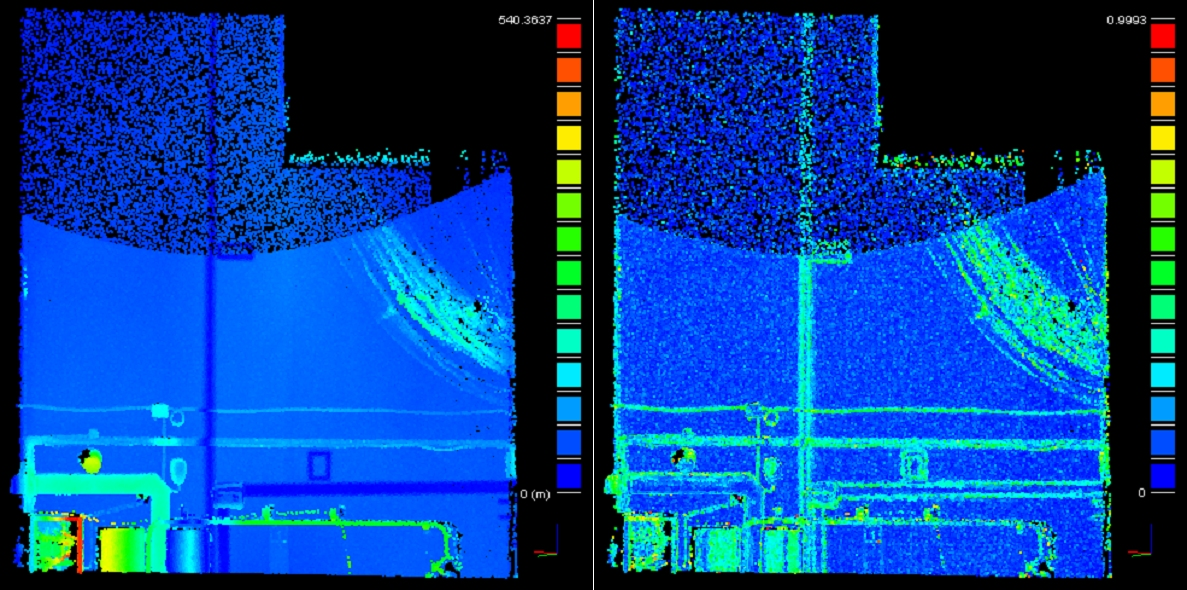
\includegraphics[width=0.6\textwidth]{Partie3_Fonctions/sfGradientExample.jpg}
\caption{\label{fig:sfGradientExample}Interface de param�tre pour le calcul des normales}
\end{center}
\end{figure}

\index{champ scalaire}
\index{gradient}
Cette fonction permet de calculer les normes du gradient du champ scalaire actif.\\
\par \emph{CloudCompare} demande � l'utilisateur de pr�ciser si le champ scalaire correspond � une distance\index{distances} euclidienne (telles que les distances calcul�es entre deux nuages ou entre un nuage et un maillage - voir~\ref{subsection:cloud2cloudDist} ou \ref{subsection:cloud2meshDist}). Si oui, l'algorithme filtrera les valeurs aberrantes (qui sont alors facilement d�tectables car dans ce cas la valeur absolue du gradient ne peut �tre sup�rieure � 1).
\\
\par
Remarques :
\begin{itemize}
\item L'algorithme cr�e un nouveau type de champ scalaire (\emph{Gradient norms}).
\item Comme pour du traitement d'image 2D classique, le gradient permet notamment de mettre en valeur les zones de fortes variations du champ scalaire (on met ainsi en �vidence les bords des zones de changement par exemple - voir
figure~\ref{fig:sfGradientExample}).
\item Comme pour du traitement d'image 2D classique, il est souvent n�cessaire d'appliquer un filtre\index{filtrage!gaussien} gaussien aux donn�es avant et/ou apr�s un calcul du gradient (Cf. section~\ref{subsection:scalarFieldGaussianFilter}).
\item Le fait que la valeur de la norme du gradient ne soit jamais sup�rieure � 1 est vrai en r�alit� pour tout champ scalaire dont les valeurs varient proportionnellement � la distance entre les points (c'est donc le cas d'un champ de distances).
\end{itemize}
